\documentclass[12pt]{article}
\usepackage[utf8]{inputenc}
\usepackage{graphicx}
\graphicspath{ {./images/} } % Uncomment
\usepackage[
top=2cm,
bottom=2cm,
left=2cm,
right=2cm,
headheight=17pt, % as per the warning by fancyhdr
includehead,includefoot,
heightrounded, % to avoid spurious underfull messages
]{geometry} 
\geometry{a4paper}
\usepackage{fancyhdr}

% Lecture Name, exercise number, group number/members
\newcommand{\lecture}{GPU Computing}
\newcommand{\exercise}{Exercise 5}
\newcommand{\groupnumber}{Group gpu04}
\newcommand{\groupmembersshort}{Pingitzer, Altuntop, Junge}
\newcommand{\groupmemberslist}{Pingitzer, Danny\\Altuntop, Ekrem\\Junge, Andreas G.}
\newcommand{\duedate}{\today}



\fancyhf{}
\fancyhead[L]{\groupnumber}
\fancyhead[R]{\textsc{\groupmembersshort}}
\fancyfoot[C]{\lecture: \exercise}
\fancyfoot[R] {\thepage}
\renewcommand{\headrulewidth}{0.4pt}
\renewcommand{\footrulewidth}{0.4pt}
\pagestyle{fancy}

\begin{document}
	\begin{titlepage}
		\centering

		{\scshape\LARGE Universität Heidelberg\\Institute for Computer Engineering (ZITI) \par}
		\vspace{1.5cm}
		{\scshape\Large Master of Science Computer Engineering \par}
		\vspace{0.5cm}
		{\scshape\Large \lecture \par}
		\vspace{1.5cm}
		{\huge\bfseries \exercise \par}
		\vspace{2cm}
		{\Large \groupnumber \itshape  \\ \groupmemberslist \par}
		\vfill
		
		
		% Bottom of the page
		{\large Due date \duedate \par}
	\end{titlepage}

\setcounter{section}{4}
\section{Exercise}
\subsection{Reading}
\emph{Read the following paper and provide review as explained in the first lecture (see slides):}\\

\noindent\emph{John Nickolls and William J. Dally. 2010. The GPU Computing Era. IEEE Micro 30, 2 (March 2010), 56-69.:}\\

\noindent @todo: Text by Ekrem.


\newpage
\subsection{Matrix Multiply – GPU na\"ive version}
\emph{Vary the threads-per-block (blocksize) parameter to determine an optimal value. Choose this parameter and report the overall runtime (sum of a,b,c) together with the different components (a,b,c) by varying	the problem size.}\\

\noindent We varied the threads-per-block parameter at the constant problem size of 1024. We found, that the optimal thread-per-block count was: 16, with an average of 26.9205 ms per Matrix Multiplication.\\
We did 10 iterations per measurement point and divided the total runtime by this, in order to have accurate results (more iterations would have been better, but would have a unacceptable runtime).\\

\begin{figure}[!htb]
	\caption{Block size from 2...32  in stepsize 2}
	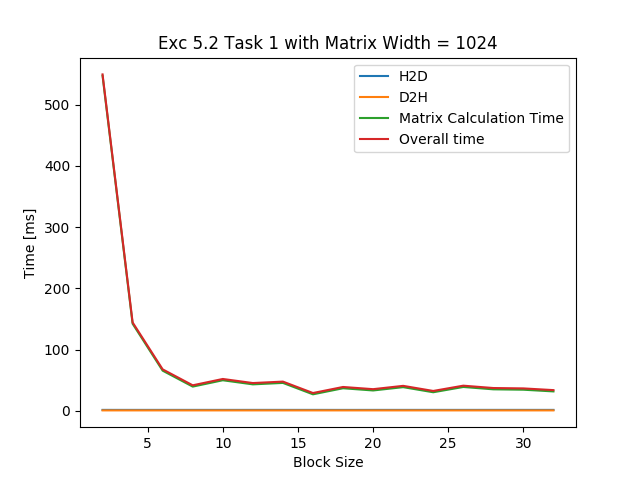
\includegraphics[scale=0.75]{5_2_01}
	\centering
\end{figure}

\newpage
\noindent With this threads-per-block number of 16, we varied the problem size (matrix size) and also compared it to sequential CPU execution time:\\

\begin{figure}[!htb]
	\caption{Matrix sizes: 16, 32, 64, 128, 256, 512, 1024, 2048, 4096, 8192}
	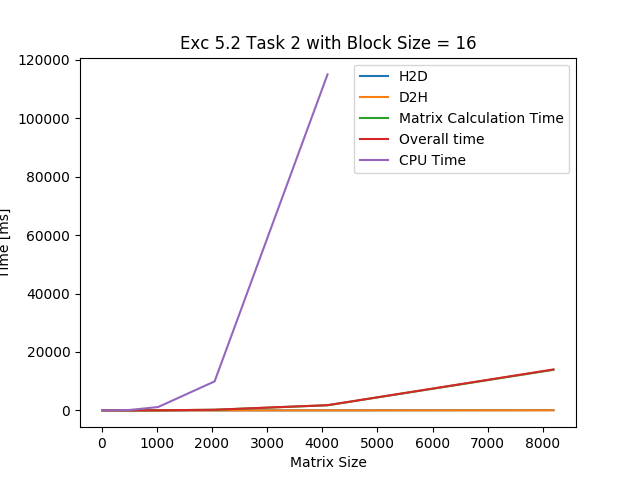
\includegraphics[scale=0.75]{5_2_02}
	\centering
\end{figure}

\noindent\emph{Report the highest speed-up you achieved compared to the CPU version from 5.2, both with and without data movements.}\\
On the CPU we could only measure up to a matrix size of 4096, everything above took too much runtime.\\
For matrix size 4096 we have:
\begin{itemize}
	\item CPU Runtime: 115026 ms
	\item GPU H2D + D2H movement time: 32.6053 ms
	\item GPU Runtime: 1755.21 ms
\end{itemize}
This is equivalent to a speedup of factor ca. 65,5 without data movements and a speedup of factor ca. 64,3 with consideration of data movement time.\\
This ratio will increase with larger matrix size.


\newpage
\subsection{Matrix Multiply – GPU version using shared memory}
\emph{Choose a suitable problem size (rather large) and vary the threads-per-block parameter to determine an optimal value. Report run time graphically.}\\
We chose a problem size of 1024 and 2048 to compare and check.\\
We found that 32 threads-per-block are optimal, with an average execution time of 19.2625 ms (for Problem Size 1024) and 151.929 ms respectively (for Problem Size 2048).\\

\begin{figure}[!htb]
	\caption{Block sizes from 2...32 in stepsize 2}
	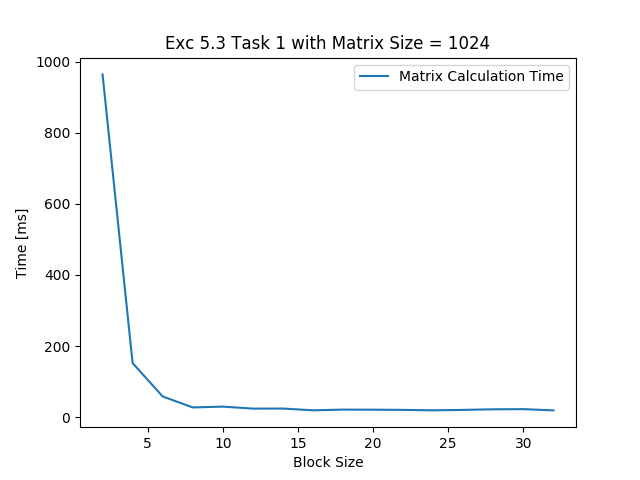
\includegraphics[scale=0.68]{5_3_01_1024}
	\centering
\end{figure}

\begin{figure}[!htb]
	\caption{Block sizes from 2...32 in stepsize 2}
	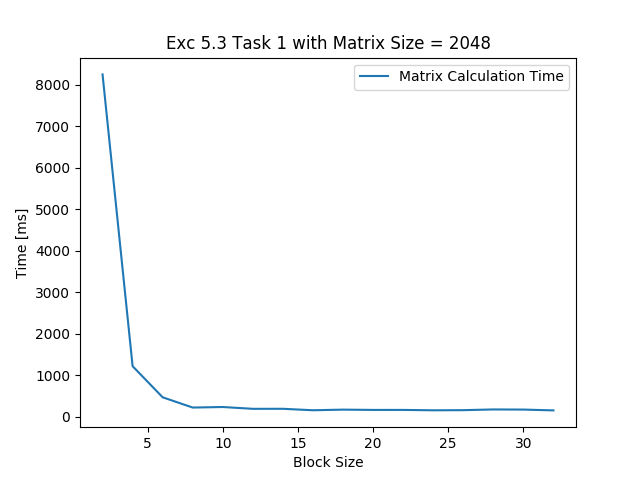
\includegraphics[scale=0.68]{5_3_01_2048}
	\centering
\end{figure}


\noindent\emph{Report the overall runtime (sum of a-c) together with the different components (a-c) by varying the problem size.}\\

\begin{figure}[!htb]
	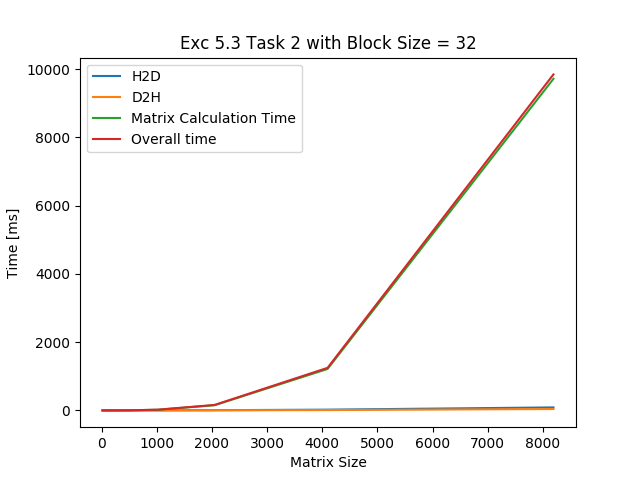
\includegraphics[scale=0.75]{5_3_02}
	\centering
\end{figure}

\noindent\emph{Report the highest speed-up you achieve compared to the two previous versions, both with and without data movements.}\\
On the CPU we could only measure up to a matrix size of 4096, everything above took too much runtime.\\
For  matrix size 4096 we have:
\begin{itemize}
	\item CPU Runtime: 115026 ms
	\item GPU H2D + D2H movement time: ca. 32 ms
	\item GPU Runtime (no shared memory): 1755.21 ms
	\item GPU Runtime (shared memory): 1214.37 ms
\end{itemize}
Speedup of shared memory version over the CPU version without data movements: 94,7 and with consideration of data movements: 92,2.
Speedup of shared memory version over the GPU non shared memory version: 1,4

\end{document}